\chapter{Propositional logic}
The definitions, lemmata, propositions and theorems as well as the notes in this chapter are sourced from \cite[chapter~1]{EndertonHerbertB2001AMIt}.
\addAbbrev{prop.}{propositional}
\defin{Language of PL}{
The Language \outernote{Language} of Propositional logic is a set containing
    \begin{itemize}
        \item logical symbols: consisting of the \graybf{sentential connective} symbols $\lnot, \land, \lor, \to, \leftrightarrow$ and parenthesis $(,)$
        \item non-logical symbols: $ A_1, A_2,A_3,\dots$ (also called sentential atoms, variables)
    \end{itemize}
    from which we assume (for unique readability) that no symbol is a finite sequence of any other symbols.
}
\note{}{
    \begin{enumerate}
        \item The role of the logical symbols doesn't change, the sentential atoms we see as variables, they function as placeholders or variables.
        \item we assumed the set of non-logical symbols is countable, for most of our conclusions you could use any set of prop. atoms of any size
    \end{enumerate}
}
\addAbbrev{exp.}{expression(s)}
\defin{Expression / prop. sentence}{An \graybf{expression}\outernote{expression}is a any finite sequence of symbols
    We define \graybf{grammatically correct exp.} recursively
    \begin{enumerate}
        \item every prop. atom is a prop. sentence
        \item if $\alpha, \beta$ are prop. sentences, then also $(\lnot \alpha), (\alpha \land \beta), (\alpha \lor \beta), (\alpha \to \beta), (\alpha \leftrightarrow \beta)$
        \item nothing else (in particular $\varnothing$ is not a prop. fla.)
    \end{enumerate}
    and call them \graybf{prop. sentences} or \graybf{prop. fla.}\outernote{prop. fla.}\outernote{prop. sentence}
    Equivalently stated every prop. sentence is built up by applying finitely many formula building operations on atoms and the prop. sent. returned from building operations.
    \[\mathcal{E}_\lnot, \mathcal{E}_\lnot(\alpha) \defeq (\lnot \alpha) \text{ for any prop. fla. $\alpha$ and similarly for } \mathcal{E}_\land,\mathcal{E}_\lor \mathcal{E}_\to, \mathcal{E}_\leftrightarrow\]
    This allows us to symbolize the \graybf{expression tree} (Here for example for $((\lnot(A_1\to A_2))\lor A_3))$
    \begin{figure}[H]
        \centering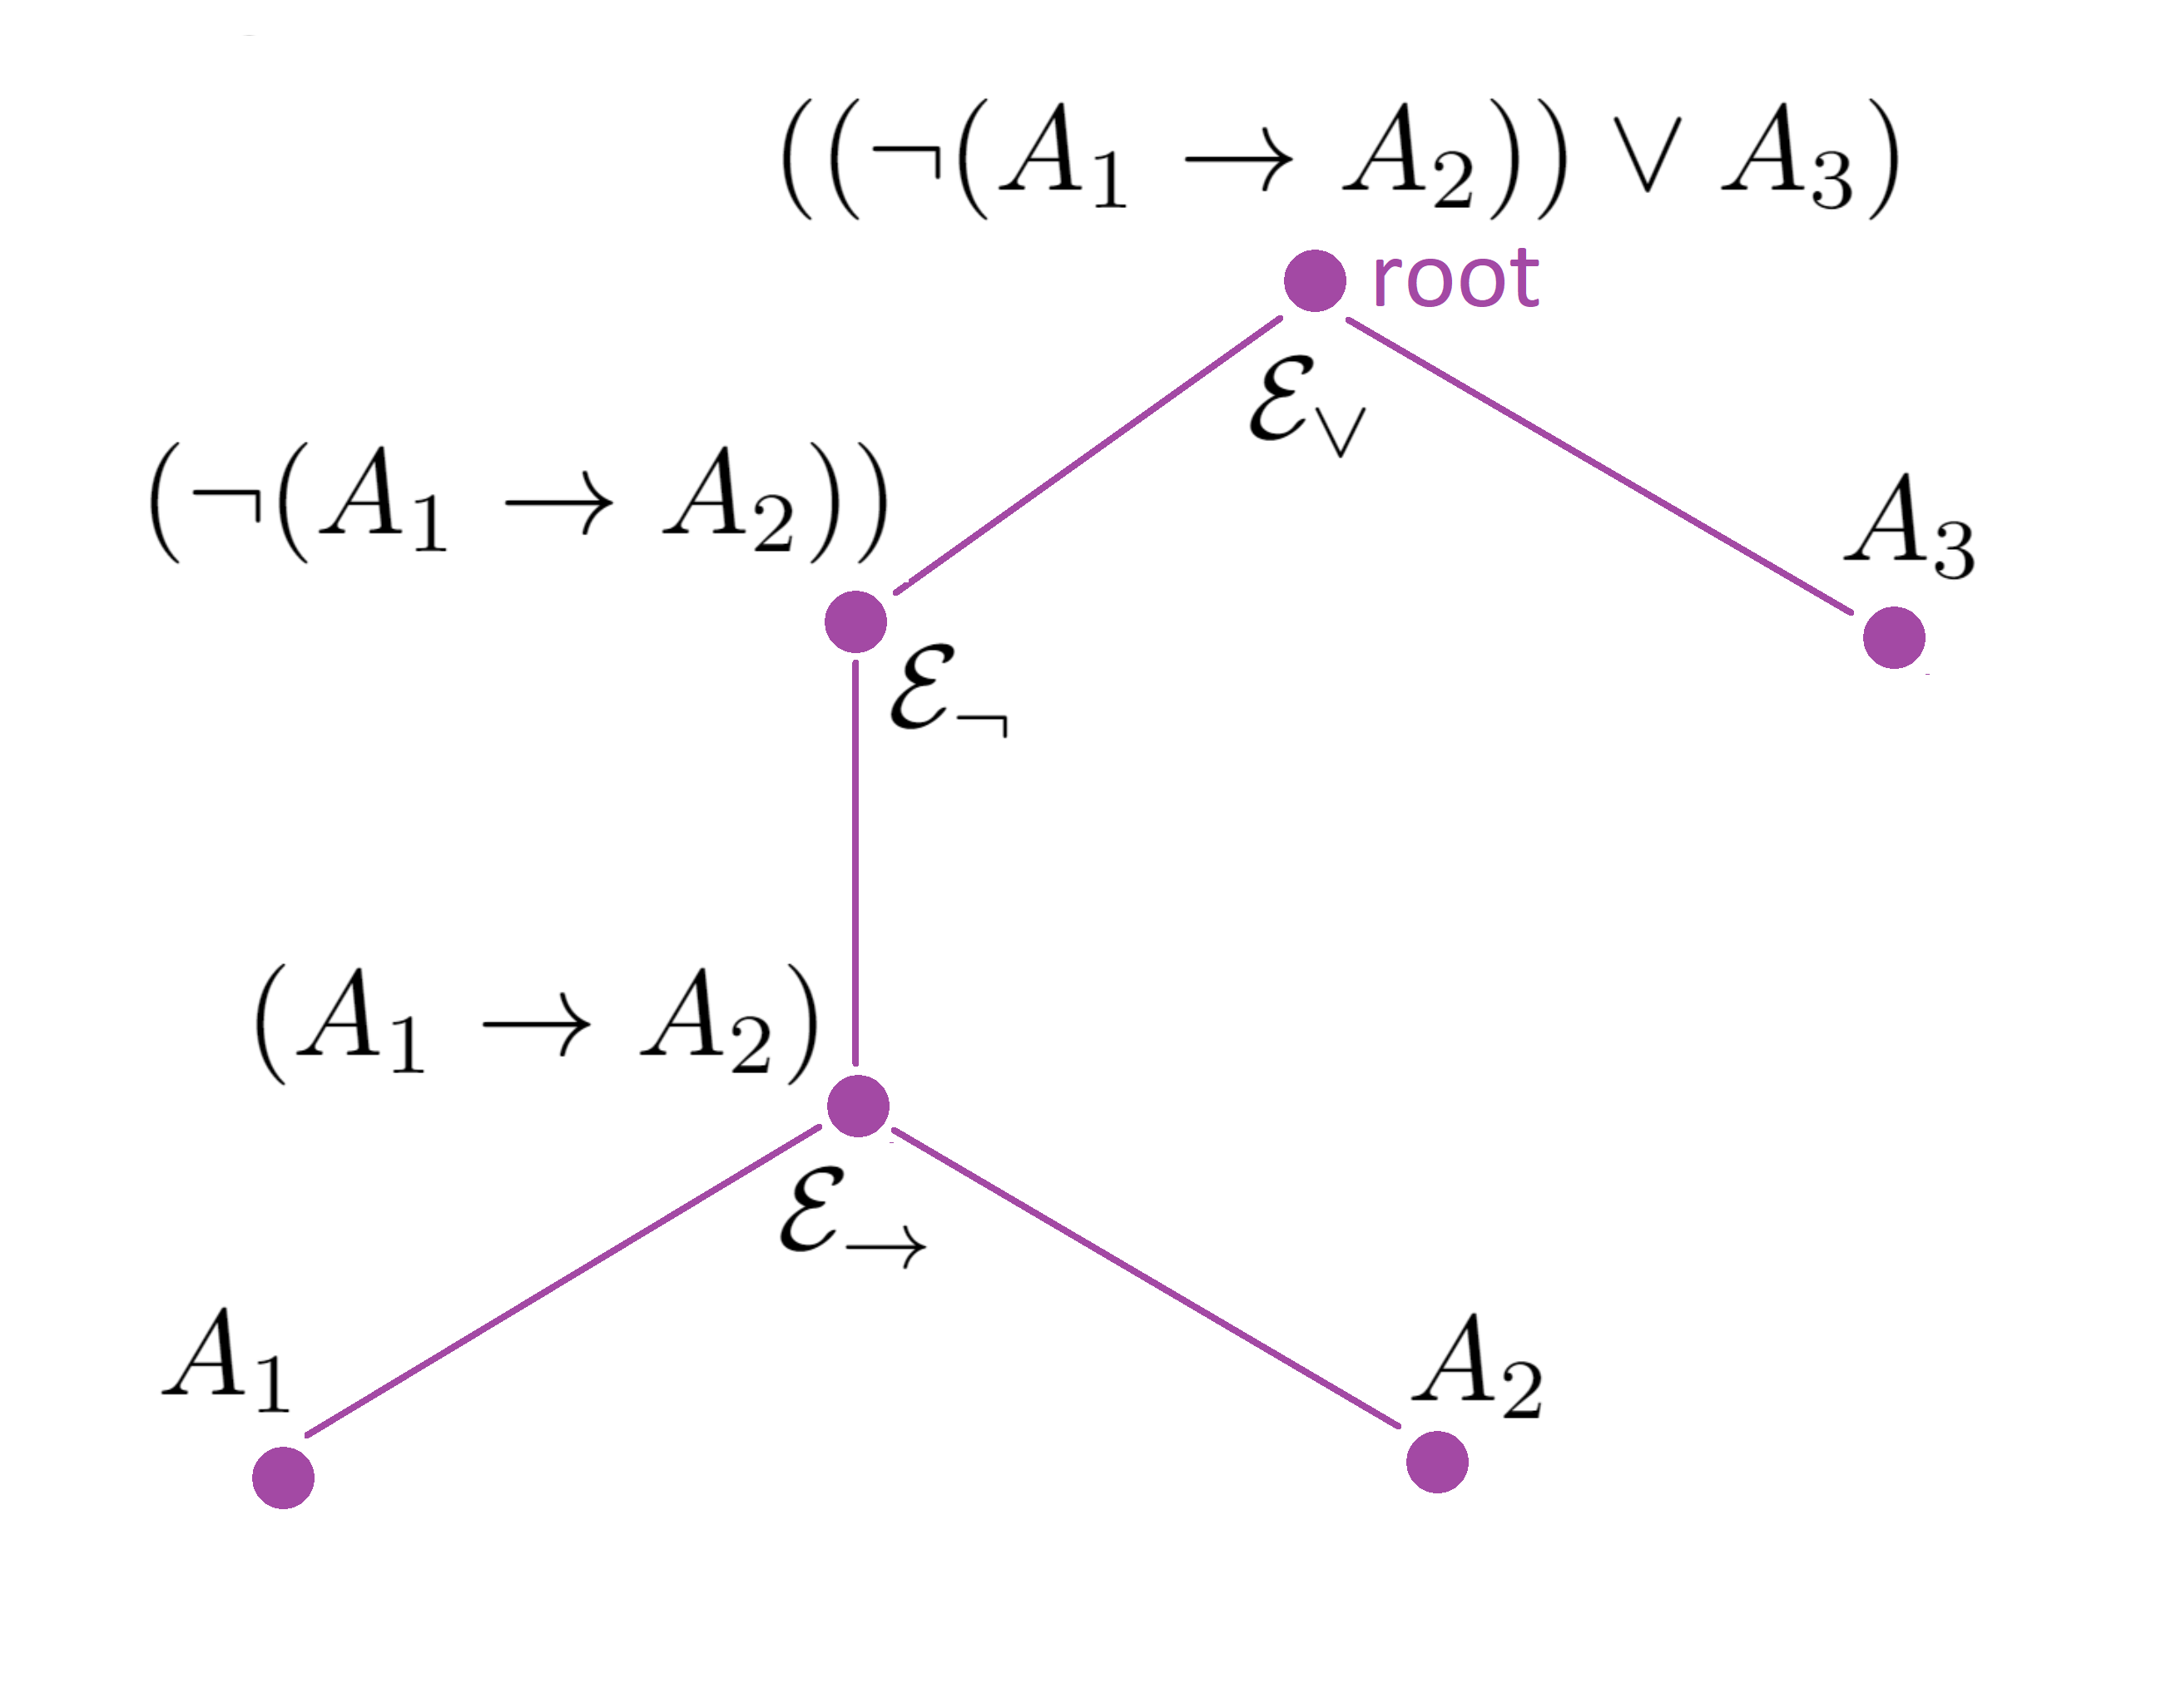
\includegraphics[width = 6cm]{1-extree.png}
    \end{figure}
    
}
We will return to these construction trees in \ref{section_parsingalg}, where we answer the question of what 
truth value a given prop. sentence might have.
\newpage
\defin{Construction sequence}{
    Given a prop. sentence $\alpha$ a \graybf{construction sequence}\outernote{construction sequence} 
    of $\alpha$ is a finite sequence $\left\langle \alpha_1,\dots \alpha_{n-1},\alpha\right\rangle$ 
    such that for all $i\leq n$
    the following holds
    \begin{itemize}
        \item $\alpha_i$ is a sentential atom
        \item or $\alpha_i= \mathcal{E}_\lnot(\alpha_j)$ for some $j< i$
        \item or $\alpha_i= \mathcal{E}_{\square }(\alpha_j,\alpha_k)$ for some $j,k<i$ and $\square\in\{\land,\lor,\to,\leftrightarrow\}$
    \end{itemize}
}
\defin{Closedness of a set}{Let $S$ be a set. We say $S$ is \graybf{closed}\outernote{closure} under an $n$-ary operational symbol $f$
    iff for all $s_1,s_2,\dots s_n\in S$ it holds $f(s_1,s_2,\dots s_n)\in S$ 
}
\addAbbrev{sent.}{sentence(s)}
\addAbbrev{seq.}{sequence}
\noindent\graybf{Induction principle:} Suppose $S$ is a set of prop. sentences
containing all prop. atoms and closed under the 5 formula building operations, 
then $S$ is the set of all prop. sentences.
\begin{proof}
    let $PS = \text{set of all prop. sent.}$
    \begin{itemize}[leftmargin=2cm]
        \item[$S\subseteq PS$:] is clear
        \item[$S\supseteq PS$:] let $\alpha\in PS$ then $\alpha$ has a construction seq. $\left\langle \alpha_1,\dots \alpha_{n-1},\alpha\right\rangle$ and $\alpha_1\in S$.
        Let's assume that for $i\leq k<n$ each $\alpha_i$ is in $S$. Then $\alpha_{k+1}$ is either an atom and therefore in $S$ or its obtained by one of the formula building operations  
        and therefore $\alpha_{k+1}\in S$
    \end{itemize}
\end{proof}
\addAbbrev{TA}{truth assignment}
\section{Truth assignments}
%We will answer the question when does a prop. sent. follow from other prop. sentences.
The interpretation of a prop. atom is either true or false, denoted by $0 / 1$ or $T / F$ or $\top / \bot$. 
A truth assigment is simply any map $\nu:S\mapsto \{0,1\}$, where $S$ is a map of propositional atoms. 
Our goal is going to be to extend any truth assigment $v$ to a function $\overline{v}: \overline{S}\mapsto \{0,1\}$, where $\overline{S}$ is the closure
of $S$ under the $5$ fla. building operations. 
\addAbbrev{fla.}{formula}
\addAbbrev{TV}{truth value}
\defin{Truth assignment}{\label{TAConditions}
Let $\{0,1\}$ be the set of truth values. \outernote{Truth assigment} A truth assignment \outernote{TA}(TA) for a set $S$ of prop. atoms is a map $\nu:S\to\{0,1\}$}
We now want to extend $\nu$ to $\overline{\nu}: \overline{S}\to \{0,1\}$, where $\overline{S}$ is the closure of $S$ under the 5 fla. building operations such that
for all propositional atoms $A\in S$ and propositional formulas $\alpha,\beta$ in $\overline{S}$
\begin{enumerate}
    \item $\overline{\nu}(A) = \nu(A)$ 
    \item $\overline{\nu}(\lnot \alpha) = 1- \nu(\alpha)$ 
    \item $\overline{\nu}(\alpha \land \beta) = \begin{cases}
        1 & \text{iff } \overline{\nu}(\alpha) = 1 = \overline{\nu}(\beta)\\
        0 & \text{otherwise}
    \end{cases}$
    \item $\overline{\nu}(\alpha \lor \beta) = \begin{cases}
        1 & \text{iff } \overline{\nu}(\alpha) = 1 \text{ or } \overline{\nu}(\beta) = 1\\
        0 & \text{otherwise}
    \end{cases}$
    \item $\overline{\nu}(\alpha \to \beta) = \begin{cases}
        1 & \text{iff } \overline{\nu}(\alpha) = 0 \text{ or } \overline{\nu}(\beta) = 1\\
        0 & \text{otherwise}
    \end{cases}$
    \item $\overline{\nu}(\alpha \leftrightarrow \beta) = \begin{cases}
        1 & \text{iff } \overline{\nu}(\alpha) =  \overline{\nu}(\beta)\\
        0 & \text{otherwise}
    \end{cases}$
\end{enumerate}
We also want the extention to be unique, that is
\thm{Unique readability}{\label{extendetTruthAss}\label{ThrmUniqueExt}
    For all TA $\nu$ for a set $S$ $\exists ! \overline{\nu}:\overline{S}\to\{0,1\}$ satisfying the above properties}{}
We will prove this later\\
\newpage
\defin{Satisfaction}{A TA $\nu$ satisfies\outernote{satisfy} a prop. sent. $\alpha$ 
    if $\overline{\nu}(\alpha)=1$ (that is, provided that everery atom of $\alpha$ is in the domain of $\nu$). 
    We call $\alpha$ satisfiable\outernote{satisfiable} if there exists a TA that satisfies it.}
\defin{Tautological implication}{\outernote{taut. implication $\models$}\addAbbrev{taut.}{tautological}
    Let $\Sigma$ be a set of prop. sent. and $\alpha$ a prop. sent. then we say:
    $\Sigma$ tautologically imlies $\alpha$ if for all TA that satisfy $\Sigma$, $\alpha$ is also satisfied and we write $\Sigma\models \alpha$.
    If $\Sigma = \{\beta\}$, we simply write $\beta \models \alpha$ If $\Sigma = \varnothing$ then $\alpha$ is called a \graybf{tautology} and we write $\models \alpha$ instead of $\varnothing \models \alpha$ \\
    $\alpha, \beta$ are called \graybf{tautologically equivalent} iff $\alpha\models \beta$ and $\beta\models \alpha$, we then write $\alpha \sledom \models \beta$
}

\note{}{In other words, tautological implication $\Sigma\models \alpha$ means that you can not find a TA, that satisfy all members of $\Sigma$ but not $\alpha$.
    A tautology is satisfied by every TA. Suppose there is no TA that satisfies $\Sigma$, then we have $\Sigma \models \alpha$ for every prop. sent. $\alpha$}
\bsp{}{$\{\lnot A \lor B\} \sledom \models A \to B$ }
\note{}{In order to check if a prop. sent. is satisfiable we need to check $2^N$ TAs, where $N=\text{\# of atoms}$. It is unknown if this can be done by an algorithm in polynomial time. Answering this 
    would settle the debate whether $P=NP$}

However we can find a way to reduce satisfiability of an infinite set $\Sigma$ of prop. sent. to all finite subsets of $\Sigma$.
There later will be a more elementary proof of the compactness theorem, this proof is not part of the exam.
\thm{Compactness theorem}{Let $\Sigma$ be an infinite set of prop. sent. such that 
    \begin{equation}\tag{finite satisfiability}
        \forall \Sigma_0 \subseteq \Sigma, \Sigma_0 \ \text{finite}\  \exists \text{ TA satisfying every member of } \Sigma_0
    \end{equation}
    then there is a TA satsfying every member of $\Sigma$.}
{
    using topology: We have our infinite set of prop. sent. which satisfies above condition. One way to look at TA is as a sequence of $0$ and $1$.
    Let $\mathcal{A} = \{A_0, A_1,\dots\}$ be the set of all prop. atoms. We are going to identify the truth assignments on $\mathcal{A}$
    with elements in $\{0,1\}^\mathcal{A}\defeq \{f: \mathcal{A}\to \{0,1\}\}$ (the set of all TAs)
    This is a topological space with product topology, on which 
    the basic open sets (called cylinders) are:
    $ U\subseteq \{0,1\}^\mathcal{A}$ is a cylinder, such that $p_n(U) = \{0,1\}$for all but finite many $n$, where $p_n$ is the $n$-th projection.
    This means $U$ is a cylinder if the truth values of its elements are at finitely many places fixed, and are arbitrary on everything else.
    
%TODO correct proof
    Note: These basic open sets are also closed.
    The open sets are unions of basic open sets.
    The idea is to use Tychonoffs Theorem which tells us that $\{0,1\}^\mathcal{A}$ is compact. i.e.
    the intersection of a family of closed subsets w/ the finite intersection property (FIP) is non-empty.
    Finite intersection property means the intersection of finitely many sets is non-empty.

    For $\alpha \in \Sigma$ let $T_\alpha \subseteq \{0,1\}^\mathcal{A}$ be the set of TA that satisfy $\alpha$.
    This $T_\alpha$ is a finite union of cylinders, hence $T_\alpha$ is closed.
    For the family $\{T_\alpha: \alpha\in\Sigma\}$ of closed sets we have (FIP). Tychonoff tells us, 
    that $\bigcup_{\alpha\in\Sigma}{T_\alpha}\neq \varnothing$ so there is a TA satisfying $\Sigma$.}
    
    For a list of tautologies: useful might be book p. 26-27
\section{A parsing algorithm}\label{section_parsingalg}
To prove \ref{extendetTruthAss} We essentially need to show that we have enough parenthesis to make the reading of a prop. sent. unique.
That is given a TA $v$ there is at most one truth value we can assign to a prop. sent.
\addAbbrev{w/}{with}
\lemma{}{Every prop. sent. has the same number of left and right parenthesis.}{
    Let $M = \text{set of prop. sent. w/ \# left parenthesis = \# right parenthesis}$ and \\
    $PS = \text{set of all prop. sent.}$
    We have $M\subseteq PS$. Since atoms have no parenthesis, they are in $M$. we just need to show that
    $M$ is closed under the 5 construction operations.\\
    $\mathcal{E}_{\lnot} = (\lnot \alpha)$ \dots
}
\newpage
\lemma{}{No proper initial segment of a prop. sent. is itself a prop. sent.}{\label{NoPropIni}
    Let $\alpha = \alpha_1\alpha_2\dots \alpha_n$ be a prop. sent. By proper initial segment we understand $\beta = \alpha_1\dots \alpha_i$ for $1\leq i<n$.    
    We will prove that every proper initial segment has an excess of left parenthesis, then we use the previous lemma.
    Let $PS = \text{set of all prop. sent.}$ and \\
    $PF = \text{set of prop. sent. s.t. no proper initial segment has \# left parenthesis = \# right parenthesis}$, 
    we will prove that these sets are the same.\\
    Let $\alpha \in PF$. By induction on the fla. building operations
    \begin{itemize}
        \item Atoms: since the empty sequence is not a prop. sent. they have no proper initial segment.
        \item If the above is true for $\alpha, \beta$ then the proper initial segments of $(\lnot \alpha)$ are of the form
        \begin{itemize}
            \item[] $(\lnot \alpha$
            \item[] $(\lnot \alpha'$ where $\alpha'$ is a propper initial segment of $\alpha$
            \item[] $($ \qquad or
            \item[] $(\lnot$
        \end{itemize}
        Therefore $\mathcal{E}_\lnot$ preserves this property and 
        under $\mathcal{E}_\land, \mathcal{E}_\lor, \mathcal{E}_\to, \mathcal{E}_\leftrightarrow$ this is also the case.
    \end{itemize}
}
\subsubsection*{Parsing algorithm}
We now give a parsing algorithm procedure. For input we take some expression $\tau$ and the algorithm will determine if $\tau$ is a prop. sent.
If so, it will generate a unique construction tree (in form of a rooted tree) for $\tau$. (i.e. the construction tree gives us unique readability)
That there is a unique way to perform the algorithm is implied by \ref{NoPropIni}
\begin{enumerate}
    \item[0.] create the root and label it $\tau$
    \item HALT if all leaves are labled w/ prop. atom and return: ``$\tau$ is a prop. sent.''
    \item select a leaf of the graph which is not labled w/ prop. atom
    \item if the first symbol of label under consideration is not a left parenthesis, then halt and return: ``$\tau$ is not a prop. sent.''
    \item if the second symbol of the label is ``$\lnot$'' then GOTO 6.
    \item scan the expression from left to right\\
    if we reach a proper initial segment of the form\addAbbrev{lp / rp}{left / right parenthesis} ``$(\beta$'' where $\# lp(\beta) = \#rp(\beta)$ and $\beta$ is followed by one of the five sentential connectives
    $\land,\lor,\to,\leftrightarrow$ and the remainder of the expression is of the form $\beta')$, where $\# lp(\beta') = \#rp(\beta')$
    \begin{itemize}
        \item [Then:] create two child nodes (left,right) to the selected element and label them (left $\defeq \beta$, right $\defeq \beta'$) GOTO 1.
        \item [Else:] HALT and return ``$\tau$ is not a prop. sent.''
    \end{itemize}
    
    \item if the expression is of the form $(\lnot \beta)$ where $\# lp(\beta) = \#rp(\beta)$
    \begin{itemize}
        \item [Then:] construct one childnode and label it $\beta$ and GOTO 1.
        \item [Else:] HALT and return: ``$\tau$ is not a prop. sent.''
    \end{itemize}
\end{enumerate}
\bsp{}{The parsing algorithm applied to $((\lnot (A_1\to A_2))\lor A_3)$ returns the following construction tree.
    \begin{center}
        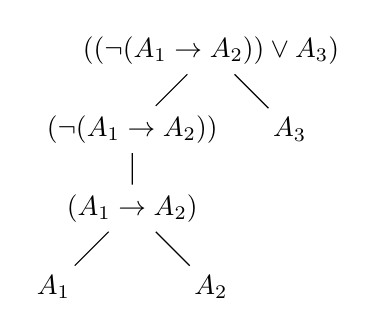
\begin{tikzpicture}
            [sibling distance=20mm, level distance=10mm]
            %\draw [help lines] (0,0) grid (-3,-3);
            \node {$((\lnot(A_1\to A_2))\lor A_3)$}
            child { node {$(\lnot(A_1 \to A_2))$}
            child { node {$(A_1 \to A_2$)} 
            child { node {$A_1$}  }
            child { node {$A_2$}  }}}
            child { node {$A_3$}};
        \end{tikzpicture}
    \end{center}
    
%    \begin{figure}[H]
%        \centering
%        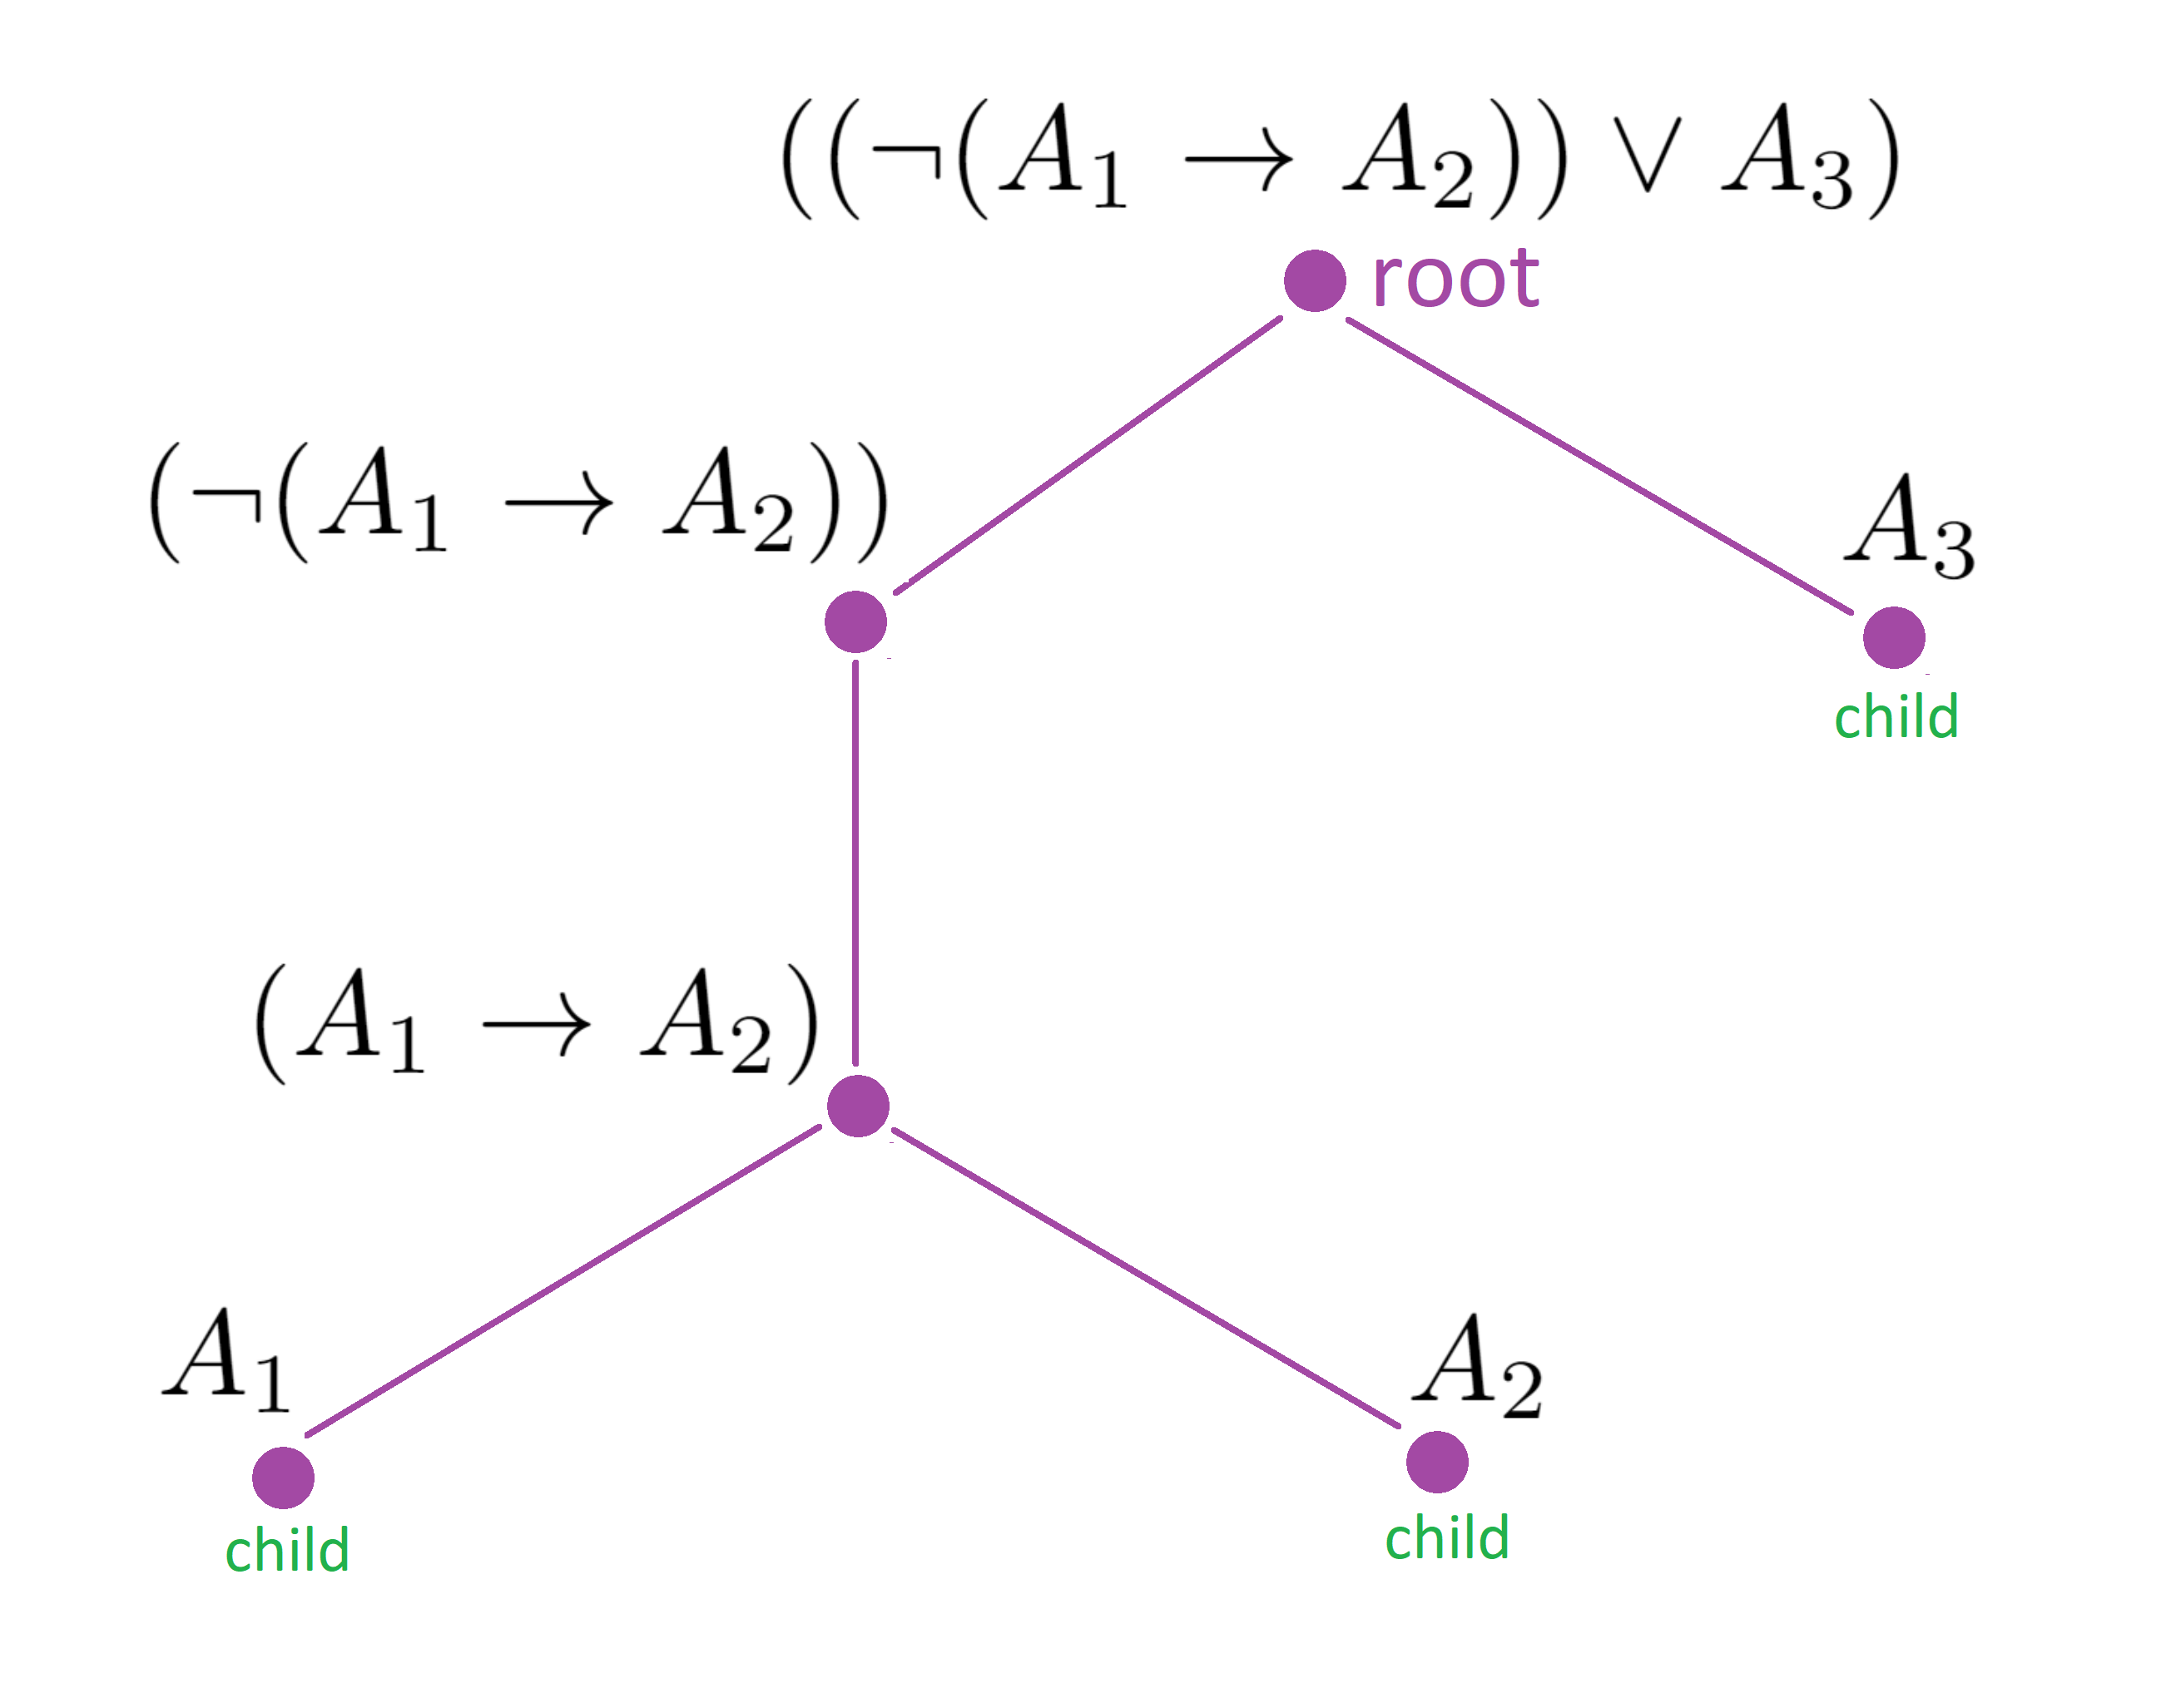
\includegraphics[width = 6cm]{1-parsing-alg-ex}
%    \end{figure}
}
\subsection*{Correctness of the parsing algorithm}
\begin{itemize}
    \item The algorithm always halts, because a child's label is shorter than the label of a parent.
    \item If the algorithm halts with the conclusion that $\tau$ is a prop. sent. 
    then we can prove inductively (starting from the leaves) that each label is a prop. sent
    \item Unique way to make choices in the algorithm: in particular $\beta, \beta'$ in step 5.
    If there was a shorter choice for $\beta$ it would be a proper initial segment of $\beta$ but such prop. sent. cannot exist.
    (This also works under the assumption that a longer choice exists).
    \item rejections are made correctly
\end{itemize}



Back to proving the existence and uniqueness of $\overline{\nu}$ in \ref{ThrmUniqueExt}.
Let $\alpha$ be a prop. sent. of $\overline{S}$. We apply the parsing algorithm to $\alpha$ to get a unique construction tree
For the leaves, use $\nu$ go get the truth values then work our way up using the conditions (1-6) in \ref{TAConditions}.
%\subsection*{A more formal notation}
\section{Induction and recursion}
\subsubsection*{Generalization of induction principle:}
Let $U$ be a set and $B\subseteq U$ our initial set.
$\mathcal{F} = \{f,g\}$ a class of functions containing just $f$ and $g$, where $$f:U\times U\to U, \qquad g: U\to U$$
We want to construct the smallest subset $C\subseteq U$ such that $B\subseteq C$ and $C$ is closed under all elements of $\mathcal{F}$.
\defin{Closedness, Inductiveness}{ We say $\mathcal{S}\subseteq U$ is 
    \begin{itemize}
        \item\graybf{closed}\outernote{closed} under $f$ and $g$ iff for all $x,y\in \mathcal{S}$ it holds $ f(x,y)\in \mathcal{S}$ and $ g(x)\in \mathcal{S}$
        \item\graybf{inductive}\outernote{inductive} if $B\subseteq \mathcal{S}$ and $\mathcal{S}$ is closed under $\mathcal{F}$
    \end{itemize}
}
\noindent One way is from the top down $$C^* \defeq\, \smashoperator{\bigcap_{\substack{B\subseteq {S}\\\text{ inductive}}}}\,{S}$$
Another is from bottom up: We call $C_1 \defeq B$, 
$$C_i \defeq C_{i-1} \cup \{f(x,y) : x,y\in C_{i-1}\}\cup \{g(x) : x\in C_{i-1}\}$$
and $C_* \defeq \bigcup_{n\geq 1}{C_{n}}$
Exercise: show that $C^* = C_*\eqdef C$.
\bsp{}{
    \begin{enumerate}
        \item Let $U$ be the set of all expressions, $B$ the set of atoms and \\
        $\mathcal{F}=\{\mathcal{E}_\square:  \square \in \{\lnot, \land,\lor,\to,\leftrightarrow \}\}$
    Then $C$ would be the set of all propositional formulas.
        \item Let $U$ be $\RR$, $B$ the set containing $0$ and $\mathcal{F}=\{S\}$, $S(x) = x+1$
        Then $C$ would be the set of the natural numbers.
    \end{enumerate}
    
}
\subsubsection*{Induction principle}
$C$ generated from $B$ by use of elements of $\mathcal{F}$ if $S\subseteq C$ such that $B\subseteq S$ and $S$ is closed under all
elements of $\mathcal{F}$, then $S = C$
\begin{proof}
    $S\subseteq C$ is clear.
    $S$ is inductive, so $C\subseteq S$.
\end{proof}

Question: under what conditions do we get ``generalized unique readability?''
The goal would be to define a function on $C$ recursively i.e. to have rules for computing $\overline{h}(x)$ for $x\in B$
with some rules of computing $\overline{h}(f(x,y))$ and $\overline{h}(g(x))$ from $\overline{h}(x)$ and $\overline{h}(y)$.
\newpage
\bsp{}{
    Suppose that $G$ is some additive group, generated from $B$ (the set of generators), 
    $h = B\to H$ where $(H,\cdot,^{-1},1)$ a group.
    When is there an extention $\overline{h}$ of $h$ s.th.
    $\overline{h}:G\to H$ is a grouphomomorphism.
    \begin{itemize}
        \item $\overline{h}(0) = 1$
        \item $\overline{h}(a+b) = \overline{h}(a)\cdot \overline{h}(b)$
        \item $\overline{h}(-a) = \overline{h}(a)^{-1}$
    \end{itemize}
    This is not always possible. \textbf{Note:} that it is possible if $G$ is generated freely by the elements of $B$ and the set of atoms is independent
    (one element of $B$ cannot be generated in finitely many steps by other elements of $B$).
}
\defin{Freely generated set}{$C$ is \graybf{freely generated}\outernote{freely generated}from $B$ by $f,g$ if 
    \begin{itemize}
        \item $C$ is generated from $B$ by $f,g$ 
        \item $f|_{C^2}$ and $g|_C$ are such that\begin{enumerate}
            \item $f|_{C^2}$ and $g|_C$ are one-to-one (injective)
            \item $\rng(f|_{C^2})$ and $\rng(g|_{C})$ and $B$ are p.w. disjoint
        \end{enumerate}
    \end{itemize}
}
\thm{Recursion Theorem}{
    $C\subseteq U$ freely generated from $B$ by $f,g$ and $V$ a set and $h:B\to V$, $F:V^2\to V$, $G:V\to V$
    Then $\exists ! \overline{h}:C\to V$ s.that 
    \begin{itemize}
        \item for all $a$ in $B$ it holds $\overline{h}(a) = h(a)$
        \item for all $x,y$ in $C$ it holds
        \begin{enumerate}
            \item $\overline{h}(f(x,y)) = F(\overline{h}(x),\overline{h}(y))$
            \item $\overline{h}(g(x)) = G(\overline{h}(x))$
        \end{enumerate}
    \end{itemize}
}{}
\note{}{if given conditions are satisfied then $h$ extends uniquely to a homomorphism 
$$(C,f,g)\to (V,F,G)$$}
Before we proof the recursion theorem, we will show how unique readability easily follows from it.

\note{}{Recusion Theorem implies unique readability for propositional formulas.
    What we need to check is that 
    the Assumptions of recursion theorem are satisfied.
    
    \textbf{Claim:} The formula building operations are one-to-one.
    \begin{claimproof}
        {$\mathcal{F}_\lor$ is one to one, suppose $(\alpha \lor \beta) = (\delta \lor \gamma)$ then $\alpha \lor \beta) = \delta \lor \gamma)$
            And $\alpha,\delta$ are prop. formulas, so they equal to each other (else one is an initial segment of the other, hence not a prop. fla.)
            By the same argument we get $\beta$ is equal to $\gamma$.
        }
    \end{claimproof}

    \textbf{Claim: }Disjointment of ranges
\begin{claimproof}
    \begin{itemize}
        \item if $(\alpha\lor \beta) = A$ then $A$ starts with $($ which can not be the case
        \item if $(\alpha\lor \beta) = (\gamma \to \delta)$ then by the same argument $\alpha$ is $\gamma$ but $\lor$ and $\to$ are diffrent
        \item if $(\alpha \lor \beta) = (\lnot \gamma)$, then $\alpha \lor \beta) = \lnot \gamma)$, so $\alpha$ would start with a $\neq$, -no
    \end{itemize}
For all other connectives the proof is similar.
\end{claimproof}
}
\subsubsection*{Proof of the Rec Thm.}
$v:C\rightharpoonup  V$ is called acceptable\outernote{acceptable} if $\forall x,y\in C$ 
\begin{enumerate}
    \item if $x\in B\cap dom(v)$ then $v(x)=h(x)$
    \item if $f(x,y)\in dom(v)$ then $x,y\in dom(v)$ and similarly for $g$
    \begin{itemize}
        \item $v(f(x,y)) = F(v(x),v(y))$
        \item $v(g(x)) = G(v(x))$
    \end{itemize}
\end{enumerate}
And when $U = \{\varGamma_v : v \text{acceptable} \}$, we define
$\overline{h}\defeq \text{function w/ graph } \bigcup \varGamma_v$
\newpage
\textbf{Claim 1:} $\overline{h}$ is a function.
\begin{claimproof}
    $$S\defeq \{x\in C : \exists \text{at most one $y$ with } (x,y)\in \bigcup \varGamma_v\}$$
    We want $S = C$, we have $S\subseteq C$,
    it is enough to show that $S$ is inductive.
    \begin{itemize}
        \item $x\in B\cap \dom(v)$ for some $v$ acceptable.\\
        then $v(x) = h(x)$ by 1.
        also $x\notin \rng (f|_{C^2})$ and $x\notin \rng (g|_C)$
        \item $x,y \in \mathcal{S}$
        We want $f(x,y),g(x)\in S$\\
        there are $v_1,v_2$ acceptable s.t. $f(x,y)\in \dom(v_1)\cap \dom(v_2)$
    \end{itemize}
\end{claimproof}
\textbf{Claim 2:} $\overline{h}$ is acceptable.
\begin{claimproof}
    $\overline{h}: C \rightharpoonup V$ by definition.
    if $x\in B\cap \dom \overline{h}$ then there is a $v$ acceptable, s.t. $x\in dom(v)$
    then $\overline{h}(x) = v(x)=h(x)$
    if $f(x,y)\in \dom \overline{h}$ then $f(x,y)\in \dom (v)$ form some $v$ acceptable.
    Hence $x,y\in \dom(v)$ and therefore $x,y\in\dom (\overline{h})$
    and we have 
    $$\overline{h}(f(x,y)) = v(f(x,y)) = F(v(x),v(y)) = F(\overline{h}(x),\overline{h}(y))$$
\end{claimproof}
\textbf{Claim 3:} The domain of $\overline{h}$ equals $C$. 
\begin{claimproof}
    it is enough to show that the domain of $\overline{h}$ is inductive. 
    $B\subseteq\dom (\overline{h})$ bc. $B\subseteq\dom (h)$ where $h$ is acceptable.
    Now we need to show closure under $f,g$. suppose $x',y'\in\dom (\overline{h})$ then $x'\in\dom (v_1)$ 
    for some acceptable $v_i$ lets assume $f(x',y')\notin\dom (\overline{h})$
    then we extend $\overline{h}$ to a function with the same graph as $\overline{h}$.
    Then
    $\varGamma \cup \{(f(x',y'),F(\overline{x'},\overline{y'}))\}$ 
    is the graph of an acceptable function.
\end{claimproof}
\textbf{Claim 4:$\overline{h}$ is uniquely constructed}
\begin{claimproof}
    Suppose both $\overline{h},\overline{\overline{h}}$ work, we schow that $S=\{x\in C: \overline{h}(x)=\overline{\overline{h}}(x)\}$ is the whole set $C$.
    it is enough to show that $S$ is inductive.
    Let $x\in B$ then $\overline{h}(x) = h(x) = \overline{\overline{h}}(x)$.
Then for $x,y\in S$ 
\[\overline{h}(f(x,y)) = F(\overline{h}(x),\overline{h}(y))=  F(\overline{\overline{h}}(x),\overline{\overline{h}}(y))=\overline{\overline{h}}(f(x,y)) \]
\[\overline{h}(g(x)) = G(\overline{h}(x))=  G(\overline{\overline{h}}(x))=\overline{\overline{h}}(g(x)) \]
and $f(x,y),g(x)\in S$, therefore $S$ is inductive.
\end{claimproof}


\section{Sentential connectives}
\defin{Tautological equivalence relation}{\outernote{tautological equivalence}For $\alpha,\beta$ prop. sent. we define $\alpha \sim \beta$ \outernote{$\sim$} \outernote{$\models \sledom$} \outernote{$\sledom \models$}
iff $\alpha \sledom\models  \beta$ (alternative notation: $\models \sledom$). This defines an equivalent relation.}
\bsp{}{$A \to B \sledom\models  \lnot A \lor B$}
\note{}{
    A $k$-place boolean function is a functon of the form $f: \{0,1\}^k\to \{0,1\}$ and we 
    define $0,1$ as the $0$-place boolean functions.\\
    If $\alpha$ is a prop. sent. then it determines a $k$-place boolean function, 
    where $k$ is the number of atoms, $\alpha$ is built up from.
    If $\alpha$ is $(A_1\lor \lnot A_2)$ then $B_\alpha: \{0,1\}^2\to \{0,1\}$ and asign its values corresponding a truth value of $\alpha$.
    That is for any TA $v:\{A_1,A_2\}\to \{0,1\}$ we define $B_\alpha(v(A_1),v(A_2)) = \overline{v}(\alpha)$
    %TODO extend / rearange function %edit 24.10. what does that mean?
}
\thm{}{If $\alpha,\beta$ are prop. sent. with at most $n$ prop. Atoms (combined), then
    \begin{enumerate}
        \item $\alpha \models \beta $ iff $\forall x\in \{0,1\}^n$ it holds $B_\alpha(x)\leq B_\beta(x)$
        \item $\alpha \sledom \models \beta $ iff $\forall x\in \{0,1\}^n$ it holds $B_\alpha(x) = B_\beta(x)$
        \item $\models \alpha $ iff $\forall x\in \{0,1\}^n$ it holds $B_\alpha(x)=1$
    \end{enumerate}
}{}
\thm{(Post)}{\footnote{Emil Post}
    Let $G$ be an $n$-ary boolean function\outernote{$n$-ary boolean func.} for $n\geq 1$. Then there is a prop. sent. $\alpha$ such that. $B_\alpha = G$.
    We say $\alpha$ realizes $G$.
}{
    \begin{enumerate}
        \item if $G$ is constantly equal to $0$ then set $\alpha$ to $A_1 \land \lnot A_1$.
        \item Otherwise the set of inputs $\{\vec{x}_1,\vec{x}_2,\dots \vec{x}_k\}$ for which $G(\vec{x}_i)=1$ holds is not empty.\\
        We denote $\vec{x}_i = (x_{i1},x_{i2},\dots x_{in})$ and define a matrix $(x_{ij})_{k\times n}$
        We further set $$\beta_{ij} = \begin{cases}
            A_j & \text{iff } x_{ij}=1\\
            \lnot A_j & \text{iff } x_{ij}=0
        \end{cases}$$\\
        \graybf{Example:} 
        \begin{equation*}
            (x_{ij})=
            \begin{pmatrix}
                0&1&0\\
                1&1&0
            \end{pmatrix}\leadsto 
            \begin{pmatrix}
                \lnot A_1 & A_2 & \lnot A_3\\
                A_1 & A_2 & \lnot A_3\\
            \end{pmatrix}=(\beta_{ij})
        \end{equation*}
        We define $\gamma_i$ as $\beta_{i1} \land \beta_{i2}\land \dots \beta_{in}$ for $1\leq i\leq k$\\
    and $\alpha$ as $\gamma_1 \lor \gamma_2\lor \dots \gamma_k = \vee_{i=1}^{k}{\gamma_i} $
    Then $B_\alpha = G$ is fulfilled.
    \end{enumerate}
}
\note{}{$\alpha$ as constructed in the proof is in the so-called Disjunctive normal form (DNF).\outernote{DNF\\ Disjunctive normal form}}
\coroll{Every prop. sent. is tautologically equivalent to a sentence in DNF}
\addAbbrev{i.e.}{id est (that is)}
\coroll{$\{\lnot,\land,\lor\}$ is a complete\outernote{complete} set of logical connectives, i.e. every prop. sent. is tautologically 
    equivalent to a sentence built up from atoms and $\lnot,\land,\lor$.
}
\thm{}{Both $\{\lnot, \land\}$ and $\{\lnot, \lor\}$ are complete.}{
    Its sufficient to show that every $k$-place boolean function is realisable by a prop. sent.
    built up using only $\lnot$ and $\land$. This is, because $\alpha\land \beta \sledom \models \lnot (\lnot \alpha \lor \lnot \beta)$
    We prove this by induction on the number of disjuctions of a prop. sent. $\alpha$ in DNF.
    Suppose the statement is true for $k \leq n$. For $n+1$ and $\alpha = \bigvee_{j=1}^{n+1}{\gamma_j}$ there exists an $\alpha' \sledom \models \bigvee_{j=1}^{n}{\gamma_j}$ and 
    $$\alpha = \bigvee_{j=1}^{n+1}{\gamma_j} \sledom \models \alpha' \lor \gamma_{n+1} \sledom \models \lnot (\lnot \alpha' \land \lnot \gamma_{n+1})$$
    %$\alpha\land \beta \sledom \models \lnot (\lnot \alpha \lor \lnot \beta)$
}
\note{}{We used the observation that, if $\alpha \sledom \models \beta$ and we replace a subsequence of $\alpha$ by a so called tautological equivalence 
    then the result is also tautologically equivalent to $\beta$}
%TODO S.10 %edit 24.10: no longer needed as is similar to proof below
\bsp{$\{\to, \land\}$ is not complete.}{Let $\alpha\in PS$ built up from only $\to,\land$ from the atoms $A_1,\dots A_n$ then we claim
    $$A_1\land A_2\land \dots \land A_n \models \alpha$$
    %Furhter we can observe that $\{\to, \lor \}$ is not complete, because if $\alpha\in PS$ is only built up from $\to,\lor$ then $\lnot \alpha$
    %can be built up from $\to, \land$. This is because of
    %$$\lnot(A\to B)\sledom \models \lnot B \to \lnot A \quad \text{and}\quad \lnot(\alpha\lor \beta) \sledom \models \lnot \alpha \land \lnot \beta$$
    We can also say $\{\to, \land\}$ is not complete bc. $\lnot A$ is not tautological equivalent to a sent. built up from $\to, \land$
    \begin{proof}
        Let $C \defeq \{\alpha \in PS \text{ built up from }\to,\land \text{ and }A_1,\dots A_n \text{ for which } \bigwedge_{i=1}^n{A_i}\models \alpha\}$
        we want to show that $C = \{\alpha \in PS \text{ built up from }\to,\land \text{ and }A_1,\dots A_n \}$
        \begin{itemize}
            \item We have $\{A_1,A_2\dots,A_n\}\subseteq C$
            \item for $\alpha,\beta\in C$ it holds
            \begin{itemize}
                \item[(1)] $A_1\land\dots\land A_n \models \alpha\to\beta$
                \item[(2)] $A_1\land\dots\land A_n \models \alpha\land \beta$
            \end{itemize}
        \end{itemize}
        Therefore $C$ is closed under the fla. building operations and we have proven our claim.
    \end{proof}
    }
\note{}{$\{\land,\lor,\to,\leftrightarrow \}$ is still not complete.}
\note{}{The number of $n$-ary boolean functions existing is $2^{2^n}$
    We define a notation for $n=0$: $\bot$ (for TV = $0$) and $\top$ (for TV = $1$)
    We can conclude that $\{\lnot,\to\}$ and $\{\to, \bot\}$ are both complete, it holds $\lnot A \sledom \models A\to \bot$
}
\defin{Satisfiability}{
    A set of prop. sent. $\Sigma$ is called \graybf{satisfiable}\outernote{satisfiable}if there exists a TA that satisfies every member of $\Sigma$.
}
\newpage
\section{Compactness Theorem}
\thm{Compactness Theorem}{\label{CompThrm}

    $\Sigma$ is satisfiable iff every finite subset $\Sigma_0\subseteq \Sigma$ is satisfiable. (i.e. $\Sigma$ is finitely satisfiable)\outernote{finitely satisfiable}}{
    Let $\Sigma$ be a finitely satisfiable set of prop. sent. Outline of the proof:
    \begin{enumerate}
        \item extend $\Sigma$ to a maximal finitely satisfiable set $\Delta$ of prop. sent.
        \item construct a thruth assigment using $\Delta$
    \end{enumerate}
    \begin{enumerate}
        \item Let $\alpha_1,\alpha_2,\dots$ be an enumeration of all prop. sent. 
        and define $\Delta_n$ inductively by $\Delta_0 \defeq \Sigma$
        $$\Delta_{n+1}\defeq \begin{cases}
            \Delta_n\cup \{\alpha_{n+1}\} & \text{if finitely satisfiable}\\
            \Delta_n\cup \{\lnot\alpha_{n+1}\} & \text{otherwise}
        \end{cases}$$
        \textbf{Claim:} $\Delta_n$ is finitely satisfiable for each $n$
        \begin{claimproof}
            By regular induction over $n$. $\Delta_0$ is finitely satisfiable. Let us assume $\Delta_n$ is finitely satisfiable.
            If $\Delta_{n+1} = \Delta_n\cup \{\alpha_{n+1}\}$ then we are finished. 
            Otherwise let $\Delta' \subseteq \Delta_n$ be a finite subset that $\Delta' \cup \{\alpha_{n+1}\}$ is not satisfiable.
            It holds $\Delta' \models \lnot \alpha_{n+1}$.
            Let us assume that $\Delta_n\cup \{\lnot\alpha_{n+1}\}$ is not finitely satisfiable. 
            Then there exists a finite subset $\Delta'' \subseteq \Delta_n $ such that $\Delta'' \cup \{\lnot\alpha_{n+1}\}$ is not satisfiable.
            It therefore holds $\Delta'' \models \alpha_{n+1}$
            But $\Delta'\cup \Delta''$ is a finite subset of $\Delta_n$ and by above observations $\Delta'\cup \Delta''\models \alpha_{n+1}$ and $\Delta'\cup \Delta''\models \lnot \alpha_{n+1}$
            A contradiction to the assumption that $\Delta_n$ is finitely satisfiable.
        \end{claimproof}
        We set $\Delta \defeq \bigcup_{i\in\NN}{\Delta_i}$ and get
        \begin{enumerate}
            \item $\Sigma\subseteq \Delta$
            \item (Maximality): for every prop. sent. $\alpha$ it holds $\alpha\in \Delta$ or $\lnot \alpha\in \Delta$
            \item (Satisfiability): $\Delta$ is finitely satisfiable. (For every finite subset there exists a $\Delta_n$ which is a superset.)
        \end{enumerate}
        \item Let $\nu$ be a TA for the prop. atoms $A_1, A_2,\dots$ such that $\nu(A) = 1$ iff $A\in \Delta$
        
        \textbf{Claim:} For every prop. sent. $\varphi$ it holds $\overline{\nu}(\varphi) =1 $ iff $\varphi\in\Delta$.
        \begin{claimproof}
            Let $S = \{\varphi \in PS \text{ s.t. } \overline{\nu}(\varphi) = 1 \text{ iff } \varphi \in \Delta\}$. \\
            \begin{itemize}
                \item $PS\supseteq S$ is clear.
                \item $PS\subseteq S$ 
                \begin{enumerate}
                    \item $\{A_1,A_2\dots\}\subseteq S$ by definition of $\nu$
                    \item closure under $\epsilon_\lnot$: Let $\varphi\in S$ then we get by maximality and satisfiability of $\Delta$: 
                    \begin{equation*}
                        \begin{split}
                            &\overline{\nu}(\lnot\varphi) = 1\\
                            \text{iff }\quad&\overline{\nu}(\varphi) = 0\\
                            \text{iff }\quad& \varphi \notin \Delta\\
                            \text{iff }\quad& (\lnot \varphi)\in \Delta
                        \end{split}
                    \end{equation*}
                    closure under $\epsilon_\to$: Let $\varphi_1,\varphi_2\in S$ similiarly
                    \begin{equation*}
                        \begin{split}
                            &\overline{\nu}(\varphi_1\to \varphi_2) = 0\\
                            \text{iff }\quad&\overline{\nu}(\varphi_1) = 1 \text{ and } \overline{\nu}(\varphi_2) = 0\\
                            \text{iff }\quad& \varphi_1 \in \Delta \text{ and }\varphi_2 \notin \Delta\\
                            \text{iff }\quad& (\varphi_1\to \varphi_2)\notin \Delta 
                        \end{split}
                    \end{equation*}
                    The closure under the other fla. building operations are similar.\qedhere
                \end{enumerate}
            \end{itemize}
        \end{claimproof}
        By this claim $\overline{\nu}$ satisfies $\Sigma$.\qedhere
    \end{enumerate}
}
\coroll{\label{CorCompThrm}
    If $\Sigma\models \tau$ then there exists a finite subset $\Sigma' \subseteq \Sigma$ s.t. $\Sigma' \models \tau$}
\begin{proof}
    Recall: $\Sigma\models \tau$ iff $\Sigma\cup\{\lnot \tau\}$ is not satisfiable.
    Suppose $\Sigma\models \tau$ but no finite subset does. \\
    Then $\forall \Sigma'\subseteq \Sigma \text{ finite } \Sigma'\cup \{\lnot \tau\}$ is satisfiable.
    By the compactness theorem $\Sigma\cup \{\lnot \tau\}$ is satisfiable which is a contradiction to $\Sigma\models \tau$.
\end{proof}
\note{}{\ref{CompThrm} and \ref{CorCompThrm} are equivalent.}

